%% ch03-qgear.tex — Chapter III: GPU-Accelerated Circuit Simulation at HPC Scale (Q-GEAR)
%% STE-edited copy (ASD-STE100 style, ~80% strictness) of chapters/ch03-qgear.tex
\chapter{GPU-Accelerated Circuit Simulation at HPC Scale}\label{ch:qgear}

This chapter addresses RQ1. It asks how far classical high-performance computing can push exact state-vector simulation of quantum circuits. It also asks how researchers with many existing \qiskit\ programs can use that capability without a rewrite for every new accelerator back end. We present \qgear, a framework that encodes \qiskit\ circuits into a few dense tensors and translates them gate by gate into \cudaq\ kernels.

We report experiments from \cite{guo2025qgear}. Random unitary circuits of up to 42 qubits were simulated on up to 1,024 NVIDIA A100 GPUs. A 34-qubit circuit that required roughly one day on a 128-core CPU node finished in about one minute on four GPUs. The same pipeline gave order-of-magnitude gains over existing GPU simulators for the Quantum Fourier transform and for \qcrank\ image-encoding circuits.

\section{Introduction and Motivation}\label{sec:qgear:intro}

Every quantum-computing research program depends on classical simulation. Before a circuit is submitted to a quantum processing unit (QPU), it is simulated:
\begin{itemize}
  \item to check that the algorithm is correct;
  \item to calibrate hyper-parameters;
  \item to estimate the shot budget;
  \item to predict which features of the output distribution should survive hardware noise.
\end{itemize}
After the hardware run, simulation gives the noiseless reference against which fidelity, energy error and success probability are measured. The difficulty is cost. An $n$-qubit circuit stores $2^{n}$ complex amplitudes and touches all of them for every gate, so both memory and time grow exponentially in $n$ (\cref{sec:bg:sim}). At $n=34$ a single-precision state vector occupies \SI{128}{\giga\byte}, and at $n=42$ it occupies \SI{32}{\tera\byte}. This exponential ``simulation wall'' is precisely what makes quantum computers interesting \cite{arute2019supremacy,preskill2018nisq}. But it also makes it difficult to develop, verify and calibrate circuits in the 30--45-qubit regime that current superconducting and trapped-ion processors can execute.

Graphics processing units (GPUs) are the natural instrument to push back this wall. A state-vector update is a memory-bound, embarrassingly data-parallel operation. It maps well to the thousands of streaming cores and the \SI{1.5}{\tera\byte\per\second} memory bandwidth of an NVIDIA A100 \cite{choquette2021a100}. NVIDIA's cuQuantum library \cite{bayraktar2023cuquantum} and the \cudaq\ programming model built on it \cite{kim2023cudaquantum} expose this hardware through kernels. The Message Passing Interface (MPI) can distribute these kernels across many GPUs. Several research simulators have shown single-GPU state-vector performance far beyond CPU back ends \cite{suzuki2021qulacs,vanbeeumen2023qclabpp,doi2023multishotgpu,asadi2024pennylanelightning}.

Yet the community's circuits are overwhelmingly written in \qiskit\ \cite{javadiabhari2024qiskit}. Its ecosystem of transpilers, hardware providers and algorithm libraries has no counterpart in the GPU-native toolchains. In our experience and that of our collaborators, a researcher who wants GPU performance has two unattractive options. The first is to rewrite the circuit in a new domain-specific language, learn its idioms and re-validate every gate. The second is to accept the CPU back end and its multi-hour turnaround.

\qgear\ removes this choice: a researcher should not have to rewrite a circuit to change the machine that simulates it. The framework accepts an ordinary \qiskit\ \texttt{QuantumCircuit} and re-materialises it as a \cudaq\ kernel at constant cost per gate, so the translation is negligible next to the simulation. The kernel runs on any available target, from a single GPU to hundreds of Perlmutter nodes. A Podman-HPC/Shifter container image captures the whole software stack, so deployment is reproducible and independent of the host.

This chapter makes the following contributions, all reported in \cite{guo2025qgear} and released as open-source software \cite{guo2025qgearsoftware}.
\begin{enumerate}
  \item A compact tensor encoding of circuit batches, with an HDF5 storage layout and JSON metadata. It decouples circuit generation from execution and ships thousands of circuits between CPU and GPU nodes as a single file (\cref{sec:qgear:encoding}).
  \item A gate-by-gate transformation from \qiskit\ gate objects to \cudaq\ kernel instructions in constant time per gate. It currently covers the gate set H, RY, RZ, U3, CX, CP, SWAP and measurement (\cref{sec:qgear:kernel}).
  \item Two execution modes. The \emph{adjoint} mode composes many sub-circuits or Hamiltonian terms into one large state-vector simulation. The \emph{parallel} mode dispatches independent circuits to independent GPUs (\cref{sec:qgear:modes}).
  \item A containerised, Slurm-integrated deployment on NERSC Perlmutter. It uses the \cudaq\ \texttt{nvidia-mgpu} target to partition a single state vector across up to 1,024 A100 GPUs by index-bit decomposition (\cref{sec:qgear:deploy}).
  \item An experimental evaluation on random unitary circuits, the Quantum Fourier transform (QFT), a variational quantum eigensolver (VQE) and \qcrank\ image-encoding circuits. It shows roughly two orders of magnitude speed-up over a 128-core CPU node, roughly one order of magnitude over existing GPU simulators, and strong scaling to 42 qubits (\cref{sec:qgear:results}).
\end{enumerate}

\section{Problem Statement and Preliminaries}\label{sec:qgear:problem}

\Cref{sec:bg:sim} gives the mathematical background of state-vector simulation. Here we fix only the notation and the cost model. An $n$-qubit pure state is a vector $\ket{\psi}\in\C^{2^{n}}$ with amplitudes $\psi_{i}$ indexed by the bit string $i=(i_{n-1}\cdots i_{1}i_{0})_{2}$, where bit $i_{q}$ is the computational-basis value of qubit $q$. A single-qubit gate $U$ on qubit $q$ updates every pair of amplitudes whose indices differ only in bit $q$,
\begin{equation}\label{eq:qgear:sqgate}
  \begin{pmatrix}\psi'_{i\,[i_{q}=0]}\\ \psi'_{i\,[i_{q}=1]}\end{pmatrix}
  = U \begin{pmatrix}\psi_{i\,[i_{q}=0]}\\ \psi_{i\,[i_{q}=1]}\end{pmatrix},
  \qquad \text{for all } 2^{n-1} \text{ such pairs},
\end{equation}
and a two-qubit gate acts analogously on quadruples of amplitudes. Every gate therefore performs $\Theta(2^{n})$ arithmetic operations and, more importantly, streams the whole state vector through memory. For a circuit with $m$ gates the time is $\Theta(m\,2^{n})$. The memory is $2^{n}\times 8$ bytes in single precision (complex64) or $2^{n}\times 16$ bytes in double precision.

Our baseline, a 128-core CPU node, has \SI{512}{\giga\byte} of DRAM and a few hundred gigabytes per second of aggregate memory bandwidth. It holds a 34-qubit single-precision state (\SI{128}{\giga\byte}), but each gate costs on the order of a second. A circuit with $10^{4}$ two-qubit gates then runs for hours. A single A100 with \SI{40}{\giga\byte} of high-bandwidth memory holds a 32-qubit single-precision state (\SI{32}{\giga\byte}) and streams it in tens of milliseconds. The same circuit therefore finishes in seconds. But each additional qubit doubles the memory, that is, the number of GPUs.

From this cost model we derive the four requirements that \qgear\ must meet.
\begin{enumerate}
  \item \emph{Transparency}: the input is a \qiskit\ circuit, and the user never writes \cudaq\ code.
  \item \emph{Negligible translation cost}: the \qiskit-to-\cudaq\ translation must be $\bigO{m}$ with a small constant, invisible next to the $\Theta(m 2^{n})$ simulation.
  \item \emph{Scalability}: the same pipeline must run on one GPU, on the four GPUs of a node and on hundreds of nodes. When the circuit is too large for one device, it must use the memory of all GPUs for a single state vector.
  \item \emph{Reproducibility}: a container must capture the software stack, and ordinary Slurm batch scripts must drive it, so that an experiment can be repeated on a different allocation or HPC centre.
\end{enumerate}

\section{Design of \qgear}\label{sec:qgear:design}

\Cref{fig:qgear:pipeline} gives an overview of the \qgear\ pipeline, from the \qiskit\ batch through the HDF5 file and the kernel builder to the GPU target.

% alt: Block diagram of the Q-GEAR pipeline. Top row: a Qiskit QuantumCircuit enters an encoder that produces three tensors (circ_type, gate_type, gate_param) which are stored in an HDF5 file with JSON metadata. Bottom row: the HDF5 file is read by a kernel builder that emits a CUDA-Q kernel, which runs on the nvidia or nvidia-mgpu target and returns results.
\begin{figure}[htbp]
\centering
\begin{tikzpicture}[
  font=\footnotesize,
  box/.style={draw,rounded corners=2pt,align=center,minimum height=10mm,inner sep=3pt,text width=26mm},
  tens/.style={draw,fill=cbSky!20,align=center,minimum height=9mm,inner sep=3pt,text width=29mm,font=\footnotesize\ttfamily},
  arr/.style={-{Latex[length=2mm]},thick}]
  % top row
  \node[box,fill=cbGray!10] (qc) at (0,0) {\qiskit\ circuits};
  \node[box] (enc) at (4.0,0) {Encoder};
  \node[tens] (t1) at (8.4,1.4) {circ\_type\\ (nCirc, 2)};
  \node[tens] (t2) at (8.4,0) {gate\_type\\ (nCirc, nGate, 3)};
  \node[tens] (t3) at (8.4,-1.4) {gate\_param\\ (nCirc, nGate, 3)};
  \node[box,fill=cbOrange!15] (h5) at (12.4,0) {HDF5 + JSON};
  \draw[arr] (qc) -- (enc);
  \draw[arr] (enc.east) -- (t1.west);
  \draw[arr] (enc.east) -- (t2.west);
  \draw[arr] (enc.east) -- (t3.west);
  \draw[arr] (t1.east) -- (h5.west);
  \draw[arr] (t2.east) -- (h5.west);
  \draw[arr] (t3.east) -- (h5.west);
  % bottom row
  \node[box] (kb) at (12.4,-3.2) {Kernel builder};
  \node[box,fill=cbGreen!15] (ker) at (8.4,-3.2) {\cudaq\ kernel};
  \node[box] (tgt) at (4.0,-3.2) {GPU target\\ \texttt{nvidia}, \texttt{nvidia-mgpu}};
  \node[box,fill=cbGray!10] (out) at (0,-3.2) {Results};
  \draw[arr] (h5) -- (kb);
  \draw[arr] (kb) -- (ker);
  \draw[arr] (ker) -- (tgt);
  \draw[arr] (tgt) -- (out);
\end{tikzpicture}
\caption{The \qgear\ pipeline. A batch of \qiskit\ circuits is encoded once into three dense tensors and stored as HDF5 with JSON metadata; a kernel builder re-materialises each circuit as a \cudaq\ kernel and executes it on a single-GPU or multi-GPU target. Schematic.}
\label{fig:qgear:pipeline}
\end{figure}

\subsection{Circuit Encoding into Pre-Allocated Tensors}\label{sec:qgear:encoding}

The first design decision separates the \emph{generation} of circuits from their \emph{execution}. Generation typically happens in \qiskit\ on a CPU login node or in a Jupyter session. Execution happens on GPU compute nodes behind the batch scheduler. Direct serialisation of \qiskit\ circuit objects, as OpenQASM text or Python pickles, is possible but slow to parse and awkward to distribute over MPI ranks. \qgear\ instead encodes a batch of $N_{\mathrm{circ}}$ circuits, each with at most $N_{\mathrm{gate}}$ gates, into three pre-allocated arrays whose shapes are known before the first gate is visited:
\begin{itemize}
  \item \texttt{circ\_type} of shape $(N_{\mathrm{circ}},2)$ and type \texttt{int32}. It holds for each circuit the pair $[\texttt{num\_qubit},\texttt{num\_gate}]$.
  \item \texttt{gate\_type} of shape $(N_{\mathrm{circ}},N_{\mathrm{gate}},3)$ and type \texttt{int32}. It holds for each gate the triple [\texttt{gate\_type}, \texttt{qubit1}, \texttt{qubit2}]. Here \texttt{gate\_type} is an integer code from the dictionary in \cref{tab:qgear:gates}, and \texttt{qubit2} is set to $-1$ for single-qubit gates.
  \item \texttt{gate\_param} of shape $(N_{\mathrm{circ}},N_{\mathrm{gate}},3)$ and type \texttt{float32}. It holds up to three real parameters per gate: $(\theta,\phi,\lambda)$ for U3, $(\theta,0,0)$ for RY, RZ and CP, and zeros for parameter-free gates.
\end{itemize}
Circuits shorter than $N_{\mathrm{gate}}$ are padded with a reserved no-operation code, so all rows have the same length. The kernel builder skips the padding with the \texttt{num\_gate} entry of \texttt{circ\_type}. The encoder makes a single pass over the \qiskit\ gate list. The encoding cost is therefore $\bigO{N_{\mathrm{circ}}N_{\mathrm{gate}}}$, with a constant dominated by attribute look-ups on the \qiskit\ objects. For the largest batches used in \cite{guo2025qgear}, with $10^{4}$ two-qubit gates per circuit, encoding takes a fraction of a second, amortised over every subsequent execution of the batch.

The three tensors are written to an HDF5 file with the same three dataset names. A JSON document stored as an HDF5 attribute records the metadata needed to interpret them:
\begin{itemize}
  \item the gate dictionary;
  \item the qubit counts;
  \item the random seed or image identifier that generated the batch;
  \item the \qiskit\ version and a time stamp.
\end{itemize}
HDF5 was chosen because it is the lingua franca of HPC data management and is readable from every language in the stack. It also supports parallel I/O from many MPI ranks and stores dense typed arrays without the parsing overhead of text formats. The encoded batch is thus a self-describing artefact. It can be regenerated deterministically, shipped to another machine, inspected with standard tools, and executed on any \cudaq\ target without the code that produced it. \Cref{app:qgear} reproduces the dataset names and the metadata schema. The exact layout is documented in \cite{guo2025qgear} and in the software repository \cite{guo2025qgearsoftware}.

\Cref{tab:qgear:gates} summarises the supported gate set and its mapping onto \cudaq\ primitives. The set is deliberately small. Together with the \qiskit\ transpiler, which can rewrite any circuit into $\{$U3, CX$\}$, it is universal. The native entries for H, RY, RZ, CP and SWAP avoid gate-count inflation. A full decomposition would cause this inflation for the QFT and \qcrank\ workloads that motivated the framework. Gates outside the set are rejected with a message that names the offending instruction and suggests the transpiler basis to use.

\begin{table}[htbp]
\caption{Gate-set coverage of \qgear\ and the mapping from \qiskit\ instructions to \cudaq\ kernel primitives. The integer code is stored in \texttt{gate\_type}; the parameter slots refer to \texttt{gate\_param}. From \cite{guo2025qgear,guo2025qgearsoftware}.}
\label{tab:qgear:gates}
\centering\small
\begin{threeparttable}
\begin{tabular}{@{}lllccl@{}}
\toprule
\qiskit\ gate & \cudaq\ primitive & Matrix / action & Qubits & Params & Notes \\
\midrule
\texttt{h}       & \texttt{h(q)}                    & Hadamard                          & 1 & 0 & Clifford \\
\texttt{ry}      & \texttt{ry(\(\theta\),q)}        & $e^{-i\theta Y/2}$                & 1 & 1 & \qcrank\ data rotations \\
\texttt{rz}      & \texttt{rz(\(\theta\),q)}        & $e^{-i\theta Z/2}$                & 1 & 1 & virtual on hardware \\
\texttt{u3}      & \texttt{u3(\(\theta,\phi,\lambda\),q)} & general $SU(2)$             & 1 & 3 & random unitaries \\
\texttt{cx}      & \texttt{cx(c,t)}                 & controlled-$X$                    & 2 & 0 & entangler \\
\texttt{cp}      & \texttt{cr1(\(\theta\),c,t)}     & $\mathrm{diag}(1,1,1,e^{i\theta})$ & 2 & 1 & QFT phases\tnote{a} \\
\texttt{swap}    & \texttt{swap(a,b)}               & exchange                          & 2 & 0 & QFT bit reversal \\
\texttt{measure} & \texttt{mz(q)}                   & $Z$-basis readout                 & 1 & 0 & to classical register \\
\bottomrule
\end{tabular}
\begin{tablenotes}\footnotesize
\item[a] \qiskit's \texttt{cp} and \cudaq's controlled \texttt{r1} share the same matrix, so no phase correction is needed.
\end{tablenotes}
\end{threeparttable}
\end{table}

\subsection{Gate-by-Gate Kernel Transformation}\label{sec:qgear:kernel}

The kernel builder reads one row of \texttt{circ\_type}, allocates a \cudaq\ qubit register of the recorded size, and then iterates over the first \texttt{num\_gate} rows of \texttt{gate\_type}. It dispatches each integer code to the corresponding kernel primitive, with the qubit indices and parameters read from the same row of \texttt{gate\_type} and \texttt{gate\_param}. The dispatch is a table look-up, and the primitive call appends one instruction to the kernel. The work per gate is therefore constant and independent of $n$, and the total translation time is $\bigO{m}$ for an $m$-gate circuit. The resulting kernel is a genuine \cudaq\ program, which the \cudaq\ just-in-time pipeline compiles once into the intermediate representation consumed by the target. The kernel can then be executed in three ways:
\begin{itemize}
  \item with \texttt{cudaq.sample}, to obtain counts;
  \item with \texttt{cudaq.observe}, to obtain expectation values of a spin operator;
  \item with \texttt{cudaq.get\_state}, to retrieve the full state vector for fidelity checks against the \qiskit\ reference on small instances.
\end{itemize}

First, the construction is \emph{lossless} for the supported gate set: every gate is mapped to a primitive with exactly the same unitary. A circuit simulated through \qgear\ therefore produces, up to floating-point rounding, the same state vector as the \qiskit\ Aer simulator on the original circuit. This was verified in \cite{guo2025qgear} on small instances by a comparison of state vectors, and on the VQE benchmark by a comparison of converged energies (\cref{sec:qgear:results-comparison}).

Second, the construction is \emph{stateless}: the builder needs only the tensors, not the original \qiskit\ objects. The encoding can therefore run on a login node. The kernel construction then runs independently on every MPI rank of a large job, with no Python objects pickled across processes.

\subsection{Workflow Modes: Adjoint and Parallel}\label{sec:qgear:modes}

Quantum-computing workloads on an HPC system come in two shapes, and \qgear\ exposes one execution mode for each (\cref{fig:qgear:modes}). In \emph{adjoint mode} a single large computation is assembled from many pieces. For instance, the cost Hamiltonian of a variational algorithm is a sum $H=H_{1}+\dots+H_{N}$ of Pauli terms, or a long circuit is the concatenation of many independently generated sub-circuits. \qgear\ composes the pieces into one kernel and one spin operator and reads all $N$ expectation values $\expval{H_{k}}$ from one state-vector simulation. When gradients are needed, adjoint differentiation \cite{jones2020adjoint} obtains them in a single backward sweep rather than by $2N$ parameter-shift evaluations. This mode benefits from the multi-GPU state-vector partitioning of \cref{sec:qgear:deploy}, because the state is large and shared.

In \emph{parallel mode} the workload consists of $N$ independent circuits. Examples are the random circuits used for benchmarking, the \qcrank\ sub-images of a large picture, and the candidate circuits of a synthesis loop (\cref{ch:synthesis}). Each MPI rank simulates its slice of the HDF5 batch on its own GPU with the single-device \texttt{nvidia} target. The ranks communicate only in the final gather of results. A single command-line flag in the Slurm script selects the mode, and both modes share the encoder, the kernel builder and the container image.

% alt: Two-row flow diagram of the Q-GEAR execution modes. Top row, adjoint mode: N pieces (Hamiltonian terms or sub-circuits) are composed into one kernel and one spin operator, run as a single state-vector simulation on the nvidia-mgpu target, and return N expectation values and adjoint gradients from one state. Bottom row, parallel mode: an HDF5 batch of N independent circuits is sliced across MPI ranks, each rank builds its own kernels and runs them on its own GPU with the nvidia target, and the results are gathered at the end.
\begin{figure}[htbp]
\centering
\begin{tikzpicture}[
  font=\footnotesize,
  box/.style={draw,rounded corners=2pt,align=center,minimum height=11mm,inner sep=2pt,text width=27mm},
  arr/.style={-{Latex[length=2mm]},thick}]
  % adjoint mode
  \node[font=\footnotesize\bfseries,anchor=south west] at (-1.45,0.75) {Adjoint mode: one large state, one simulation};
  \node[box,fill=cbGray!10]   (a1) at (0,0)    {$N$ pieces:\\ $H_{1},\dots,H_{N}$\\ or sub-circuits};
  \node[box,fill=cbSky!20]    (a2) at (3.6,0)  {one kernel +\\ one spin operator};
  \node[box,fill=cbGreen!15]  (a3) at (7.2,0)  {one state-vector\\ simulation\\ \texttt{nvidia-mgpu}};
  \node[box,fill=cbOrange!15] (a4) at (10.8,0) {$N$ values $\expval{H_{k}}$\\ + adjoint gradients\\ from one state};
  \draw[arr] (a1) -- (a2);
  \draw[arr] (a2) -- (a3);
  \draw[arr] (a3) -- (a4);
  % parallel mode
  \node[font=\footnotesize\bfseries,anchor=south west] at (-1.45,-2.05) {Parallel mode: $N$ independent circuits, one GPU each};
  \node[box,fill=cbGray!10]   (p1) at (0,-2.8)    {HDF5 batch of\\ $N$ independent\\ circuits};
  \node[box,fill=cbSky!20]    (p2) at (3.6,-2.8)  {MPI rank $r$ reads\\ slice $r$ and builds\\ its own kernels};
  \node[box,fill=cbGreen!15]  (p3) at (7.2,-2.8)  {GPU $r$ simulates\\ slice $r$\\ \texttt{nvidia} target};
  \node[box,fill=cbOrange!15] (p4) at (10.8,-2.8) {final gather\\ of results};
  \draw[arr] (p1) -- (p2);
  \draw[arr] (p2) -- (p3);
  \draw[arr] (p3) -- (p4);
  \node[font=\scriptsize,cbGray,anchor=north] at (5.4,-3.95) {no inter-rank communication before the final gather};
\end{tikzpicture}
\caption{The two execution modes of \qgear. Adjoint mode composes $N$ Hamiltonian terms or sub-circuits into one kernel and one spin operator and runs a single state-vector simulation on the \texttt{nvidia-mgpu} target, so all $N$ expectation values and their adjoint gradients come from one state. Parallel mode gives each MPI rank a slice of the HDF5 batch to simulate on its own GPU with the \texttt{nvidia} target and gathers the results at the end. Schematic.}
\label{fig:qgear:modes}
\end{figure}

\subsection{Containerised Deployment and Multi-GPU Execution}\label{sec:qgear:deploy}

Reproducible deployment on a shared HPC system is also a software-engineering problem. The \cudaq\ tool-chain depends on a specific CUDA driver interface and a specific MPI implementation. It also needs a Python environment that matches the \qiskit\ version used to generate the circuits. \qgear\ freezes this stack in an Open Container Initiative image derived from the official \cudaq\ image, with \qiskit, h5py and the \qgear\ package added. It runs the image through Podman-HPC on Perlmutter \cite{stephey2022podman}. Shifter images are produced from the same definition for systems that do not support Podman-HPC.

Slurm launches the image with one task per GPU, and its plugin exposes the Cray MPICH libraries of the host to the container. The containerised \cudaq\ runtime can therefore use the Slingshot interconnect directly rather than fall back to TCP. A typical job script requests $R$ GPU nodes, sets the \cudaq\ target to \texttt{nvidia-mgpu}, and launches $4R$ ranks with \texttt{srun}. The same script with the target set to \texttt{nvidia} runs the parallel mode. The Slurm scripts, image definitions and environment files are part of the released software \cite{guo2025qgearsoftware} and are listed in \cref{app:qgear}.

The \texttt{nvidia-mgpu} target distributes one state vector over $G=2^{g}$ GPUs by \emph{index-bit partitioning}, shown in \cref{fig:qgear:partition}. Write the amplitude index as $i=(i_{n-1}\cdots i_{0})_{2}$. The $g$ most significant bits $(i_{n-1}\cdots i_{n-g})$ select the GPU that owns the amplitude. The remaining $n-g$ bits are its offset inside that GPU's local array of $2^{n-g}$ elements. Each GPU therefore stores a contiguous block of $2^{n-g}$ amplitudes, or $2^{n-g}\times 8$ bytes in single precision. Qubits $0,\dots,n-g-1$ are called \emph{local} and qubits $n-g,\dots,n-1$ are called \emph{global}.

On A100 GPUs with \SI{40}{\giga\byte} this bounds the local block to $2^{32}$ amplitudes, so $G$ GPUs can hold at most $n = 32+g$ qubits. This gives 32 qubits on one GPU, 34 on the four GPUs of a node, 36 on four nodes, and 42 on $2^{10}=1,024$ GPUs. The last is the largest configuration reported in \cite{guo2025qgear}.

The partition determines which gates need communication. A single-qubit gate on a local qubit $q<n-g$ pairs amplitudes whose indices differ only in bit $q$, so both have the same top $g$ bits and live on the same GPU. The update in \cref{eq:qgear:sqgate} is then entirely local, and all $G$ GPUs proceed in parallel with no data movement.

A single-qubit gate on a global qubit $q\geq n-g$ pairs amplitudes whose GPU ranks differ in bit $q-(n-g)$. Every GPU must then exchange half of its block, $2^{n-g-1}$ amplitudes, with its partner GPU before the update can be applied. \cudaq\ implements this as a pairwise exchange over NVLink within a node and over the Slingshot network between nodes. When several global gates follow one another, it instead permutes the qubit ordering, which turns global qubits into local ones and back.

Two-qubit gates follow the same rule for each of their qubits, with one simplification for controlled gates. If only the \emph{control} qubit is global, no exchange is needed. The gate is the identity on the GPUs whose rank bit is 0 and the target operation on those whose rank bit is 1. Only a global \emph{target} qubit forces communication.

The communication volume per global gate is $2^{n-g-1}\times 8$ bytes per GPU, which for a 42-qubit state on 1,024 GPUs is \SI{16}{\giga\byte} per GPU and per gate. The measured GPU utilisation nevertheless stayed near 100\% (\cref{sec:qgear:results-scaling}). This reflects the high bandwidth of NVLink and Slingshot. It also reflects that only the $g$ global qubits, a small minority of the $n$ qubits in a random circuit, ever trigger an exchange.

% alt: Schematic of index-bit partitioning of a 2^n state vector across four GPUs. A horizontal strip of amplitudes is divided into four colored blocks labelled GPU 0 to GPU 3 by the two most significant index bits. Below, the index bit field is split into a GPU-rank part (g bits) and a local-offset part (n-g bits). A short double arrow inside one block shows that a gate on a local qubit pairs amplitudes within a GPU; a long arc between GPU 0 and GPU 2 shows that a gate on a global qubit pairs amplitudes on different GPUs and requires communication.
\begin{figure}[htbp]
\centering
\begin{tikzpicture}[font=\footnotesize, arr/.style={{Latex[length=1.6mm]}-{Latex[length=1.6mm]},thick}]
  % amplitude strip split over G = 4 GPUs
  \foreach \g/\c/\b in {0/cbBlue/00, 1/cbOrange/01, 2/cbGreen/10, 3/cbRed/11} {
    \draw[fill=\c!20,draw=\c,thick] (\g*3.3,0) rectangle ++(3.3,0.9);
    \node at (\g*3.3+1.65,0.62) {GPU \g};
    \node[font=\scriptsize] at (\g*3.3+1.65,0.25) {$i_{n-1}i_{n-2}=\b$, $2^{n-2}$ ampl.};
  }
  \node[anchor=south west,font=\footnotesize] at (9.6,1.05) {$\ket{\psi}\in\C^{2^{n}}$, $G=4$ GPUs};
  % local gate arrow inside GPU 0
  \draw[arr,cbBlue] (0.5,1.05) to[bend left=50] (1.5,1.05);
  \node[font=\scriptsize,cbBlue,anchor=south west] at (0.0,1.35) {local qubit $q<n-g$: both amplitudes on one GPU};
  % global gate arrow between GPU 0 and GPU 2
  \draw[arr,cbRed] (2.4,-0.15) to[bend right=25] (7.4,-0.15);
  \node[font=\scriptsize,cbRed,anchor=north] at (5.0,-0.85) {global qubit $q=n-1$: partner on another GPU (exchange $2^{n-g-1}$ amplitudes)};
  % bit field
  \begin{scope}[yshift=-2.5cm]
    \draw[thick] (1.8,0) rectangle ++(1.3,0.7); \node at (2.45,0.35) {$i_{n-1}$};
    \draw[thick] (3.1,0) rectangle ++(1.3,0.7); \node at (3.75,0.35) {$i_{n-2}$};
    \draw[thick] (4.4,0) rectangle ++(1.3,0.7); \node at (5.05,0.35) {$i_{n-3}$};
    \draw[thick] (5.7,0) rectangle ++(3.6,0.7); \node at (7.5,0.35) {$\cdots$};
    \draw[thick] (9.3,0) rectangle ++(1.3,0.7); \node at (9.95,0.35) {$i_{1}$};
    \draw[thick] (10.6,0) rectangle ++(1.3,0.7); \node at (11.25,0.35) {$i_{0}$};
    \draw[decorate,decoration={brace,mirror,amplitude=5pt}] (1.8,-0.1) -- (4.4,-0.1) node[midway,below=6pt] {GPU rank ($g=2$ bits)};
    \draw[decorate,decoration={brace,mirror,amplitude=5pt}] (4.4,-0.1) -- (11.9,-0.1) node[midway,below=6pt] {local offset ($n-g$ bits)};
    \node[anchor=east] at (1.6,0.35) {index $i$:};
  \end{scope}
\end{tikzpicture}
\caption{Index-bit partitioning of a $2^{n}$-amplitude state vector over $G=2^{g}$ GPUs (here $G=4$). The $g$ most significant index bits select the GPU and the remaining $n-g$ bits address the amplitude inside the GPU's block. Gates on local qubits need no communication; gates whose target is a global qubit require each GPU to exchange half of its block with a partner. Schematic.}
\label{fig:qgear:partition}
\end{figure}

\section{Implementation}\label{sec:qgear:impl}

\qgear\ is a Python package built with the nbdev literate-programming tool-chain, so the documentation, the unit tests and the source come from the same notebooks \cite{guo2025qgearsoftware}. The package has three modules that mirror \cref{fig:qgear:pipeline}:
\begin{itemize}
  \item an encoder module that walks a \qiskit\ circuit and fills the three tensors;
  \item an I/O module that writes and reads the HDF5 batch file with its JSON metadata;
  \item a kernel-builder module that produces \cudaq\ kernels and wraps the \texttt{sample}, \texttt{observe} and \texttt{get\_state} entry points.
\end{itemize}
A command-line driver combines them with argument parsing for the target, the mode, the shot count and the batch slice assigned to the current MPI rank. Example generators cover the benchmark families of this chapter: random CX-block circuits, QFT, VQE ans\"atze and \qcrank\ image encoders built on the encoder of \cite{balewski2024qcrank}. The Jupyter notebooks that produced the figures of \cite{guo2025qgear} are included for reproducibility.

All GPU experiments were run on the Perlmutter system at NERSC (\cref{fig:qgear:perlmutter}). A GPU node has one AMD EPYC 7763 ``Milan'' processor and four NVIDIA A100 GPUs with \SI{40}{\giga\byte} of HBM2 each, fully connected by third-generation NVLink. PCIe Gen4 links the GPUs to the CPU, and four HPE Slingshot~11 (Cassini) network interface cards give every GPU its own path to the interconnect. The baseline CPU node has two AMD EPYC 7763 processors (128 cores) and \SI{512}{\giga\byte} of DDR4. The \SI{40}{\giga\byte} GPU memory sets the 32-qubits-per-GPU limit of \cref{sec:qgear:deploy}, and the NVLink and Slingshot bandwidths make the exchange of global-qubit amplitudes affordable.

% alt: Two side-by-side block diagrams. Left: a Perlmutter CPU node with two AMD EPYC 7763 processors sharing 512 GB DDR4 and one Slingshot NIC. Right: a Perlmutter GPU node with one AMD EPYC 7763 processor connected by PCIe Gen4 to four A100 40 GB GPUs that are interconnected by NVLink, each GPU paired with a Slingshot 11 (Cassini) NIC.
\begin{figure}[htbp]
\centering
\begin{tikzpicture}[font=\scriptsize,
  cpu/.style={draw,fill=cbGray!15,rounded corners=2pt,align=center,minimum width=22mm,minimum height=9mm},
  gpu/.style={draw,fill=cbGreen!20,rounded corners=2pt,align=center,minimum width=16mm,minimum height=8mm},
  mem/.style={draw,fill=cbOrange!15,align=center,minimum width=22mm,minimum height=6mm},
  nic/.style={draw,fill=cbSky!25,align=center,minimum width=16mm,minimum height=7mm},
  lnk/.style={thick}]
  % ---- CPU node ----
  \begin{scope}
    \node[draw,dashed,rounded corners=3pt,minimum width=54mm,minimum height=50mm] (cpubox) at (0,0) {};
    \node[anchor=north,font=\footnotesize\bfseries] at (cpubox.north) {CPU node (baseline)};
    \node[cpu] (c1) at (-1.5,0.9) {AMD EPYC 7763\\ 64 cores};
    \node[cpu] (c2) at (1.5,0.9) {AMD EPYC 7763\\ 64 cores};
    \node[mem,minimum width=50mm] (m1) at (0,-0.55) {\SI{512}{\giga\byte} DDR4 (shared)};
    \node[nic] (n1) at (0,-1.7) {Slingshot 11\\ NIC};
    \draw[lnk] (c1) -- (c2);
    \draw[lnk] (c1.south) -- (m1.north -| c1.south);
    \draw[lnk] (c2.south) -- (m1.north -| c2.south);
    \draw[lnk] (m1) -- (n1) node[midway,right=1pt,font=\tiny] {PCIe Gen4};
  \end{scope}
  % ---- GPU node ----
  \begin{scope}[xshift=8.4cm]
    \node[draw,dashed,rounded corners=3pt,minimum width=82mm,minimum height=50mm] (gpubox) at (0,0) {};
    \node[anchor=north,font=\footnotesize\bfseries] at (gpubox.north) {GPU node};
    \node[cpu,minimum width=40mm] (hc) at (0,1.55) {AMD EPYC 7763 (Milan), 64 cores, \SI{256}{\giga\byte} DDR4};
    \foreach \k/\x in {0/-2.85,1/-0.95,2/0.95,3/2.85} {
      \node[nic] (n\k) at (\x,0.35) {Slingshot 11\\ NIC \k};
      \node[gpu] (g\k) at (\x,-0.75) {A100 \k\\ \SI{40}{\giga\byte}};
      \draw[lnk,cbGray] (hc.south) -- (n\k.north);
      \draw[lnk,cbGray] (n\k.south) -- (g\k.north);
    }
    \node[font=\tiny,cbGray,anchor=west] at (3.0,0.95) {PCIe Gen4};
    % NVLink bus below the GPUs
    \draw[line width=2pt,cbGreen!70!black] (-3.6,-1.55) -- (3.6,-1.55);
    \foreach \k in {0,1,2,3} {\draw[lnk,cbGreen!70!black] (g\k.south) -- (g\k.south |- 0,-1.55);}
    \node[font=\tiny,cbGreen!70!black,anchor=north] at (0,-1.6) {NVLink 3, all-to-all among the four GPUs};
  \end{scope}
\end{tikzpicture}
\caption{Perlmutter node types used in this chapter. Left: CPU node with two AMD EPYC 7763 processors (128 cores) and \SI{512}{\giga\byte} of DDR4. Right: GPU node with one AMD EPYC 7763 processor, four NVIDIA A100 GPUs with \SI{40}{\giga\byte} each connected by NVLink, PCIe Gen4 host links and four Slingshot~11 (Cassini) network interfaces. Schematic based on the system description in \cite{guo2025qgear}.}
\label{fig:qgear:perlmutter}
\end{figure}

\Cref{tab:qgear:env} summarises the software environment. The container is based on the official \cudaq\ image and adds a conda environment on the Perlmutter \texttt{/pscratch} file system. The Python packages are therefore read from the fast parallel file system rather than from the container layer at every rank start-up. This detail matters when a job launches 1,024 ranks that all import \qiskit\ and h5py within the same second. The CPU baseline runs the \qiskit\ Aer state-vector simulator with OpenMP threading over the 128 cores of a CPU node. It is subject to the 24-hour wall-clock limit of the Perlmutter regular queue.

\begin{table}[htbp]
\caption{Hardware and software environment of the \qgear\ experiments. From \cite{guo2025qgear,guo2025qgearsoftware}; version numbers not stated in the summary are marked.}
\label{tab:qgear:env}
\centering\small
\begin{tabular}{@{}lp{0.62\linewidth}@{}}
\toprule
Component & Configuration \\
\midrule
System & NERSC Perlmutter (HPE Cray EX); TTU HPCC for development runs \\
GPU node & $1\times$ AMD EPYC 7763, $4\times$ NVIDIA A100 \SI{40}{\giga\byte} (NVLink), PCIe Gen4, $4\times$ Slingshot~11 \\
CPU node (baseline) & $2\times$ AMD EPYC 7763 (128 cores), \SI{512}{\giga\byte} DDR4 \\
Largest GPU job & 256 GPU nodes, 1,024 A100 GPUs, 42 qubits \\
Scheduler & Slurm, one MPI rank per GPU, 24-hour wall-clock limit on the CPU queue \\
Containers & Podman-HPC (Perlmutter); Shifter image built from the same definition \\
GPU simulator & \cudaq\ with cuQuantum \texttt{custatevec}; targets \texttt{nvidia}, \texttt{nvidia-mgpu} (\texttt{cudaq} from PyPI as required by \texttt{qgear}~1.1.2; the paper does not pin a version) \\
CPU simulator & \qiskit\ Aer state-vector (\texttt{qiskit} and \texttt{qiskit-aer} from PyPI, unpinned) \\
Other GPU baselines & \qiskit\ Aer GPU; PennyLane Lightning-GPU \\
Language / environment & Python 3.11; conda environment on \texttt{/pscratch}; h5py for HDF5 I/O \\
Precision & complex64 (single) state vector, $2^{32}$ amplitudes per GPU \\
\bottomrule
\end{tabular}
\end{table}

\section{Experimental Setup}\label{sec:qgear:setup}

The evaluation in \cite{guo2025qgear} uses four families of circuits that exercise different aspects of the pipeline.
\begin{enumerate}
  \item \emph{Random CX-block circuits}: layers of random U3 rotations on all qubits interleaved with CX gates on randomly chosen pairs, with $n$ from 28 to 34 qubits and 100 to 10,000 two-qubit gates. They have no structure that a simulator could exploit, so they measure the raw state-vector throughput of each back end. Circuits with 100 two-qubit gates are \emph{short}, those with 10,000 \emph{long}.
  \item The \emph{Quantum Fourier transform} on up to 22 qubits. Its $\Theta(n^{2})$ controlled-phase gates and final SWAP layer make it a standard structured benchmark and a component of many algorithms.
  \item An 18-qubit \emph{VQE} instance, which exercises the adjoint mode. An optimiser calls the simulator repeatedly for expectation values of a many-term Hamiltonian, so per-call latency rather than raw throughput dominates.
  \item \emph{\qcrank\ image encoding} \cite{balewski2024qcrank}. A grey-scale image of $2^{n_{a}}\times n_{d}$ pixels is loaded into $n_{a}$ address and $n_{d}$ data qubits by uniformly controlled rotations. The pixel values are recovered from many measurements of the circuit. This family represents the data-encoding workloads of \cref{ch:qml} and requires millions of shots, which stresses the sampling path rather than the gate-application path.
\end{enumerate}

Each configuration was timed end to end, from kernel construction to the availability of the result in Python. The CPU baseline was run on a dedicated CPU node under the 24-hour limit. A CPU run that did not finish within the limit is reported as exceeding \SI{24}{\hour}. GPU utilisation was recorded with the NVIDIA system-management interface. For the multi-node runs the number of GPUs was first set to the smallest power of two that holds the state ($G=2^{n-32}$). It was then increased to measure strong scaling at fixed $n$. Correctness was checked on small instances by a comparison of state vectors between \qgear\ and \qiskit\ Aer. For the VQE, the converged energy was compared with the exact ground-state energy.

\section{Results}\label{sec:qgear:results}

\subsection{CPU Versus GPU on Random Circuits}\label{sec:qgear:results-cpu-gpu}

\Cref{fig:qgear:cpu-gpu} compares the simulation time of short and long random circuits on the CPU node, one A100 and the four A100s of one GPU node. The headline numbers from \cite{guo2025qgear} follow. A 34-qubit long random unitary took approximately \SI{24}{\hour} on the 128-core CPU node, that is, the entire wall-clock allowance. The same circuit finished in approximately \SI{1}{\minute} on four A100 GPUs with the \texttt{nvidia-mgpu} target. On a single A100, which holds circuits of up to 32 qubits, the speed-up over the CPU node was approximately $400\times$.

The GPU curves follow the expected $2^{n}$ slope: each additional qubit roughly doubles the time, because each gate streams a state vector of twice the size. The CPU curve rises somewhat faster than $2^{n}$ once the state exceeds the last-level caches and the memory-bandwidth limit of the socket dominates. For short circuits the GPU times are nearly flat in $n$. Fixed costs dominate these times rather than gate application: chiefly kernel compilation, state allocation and the transfer of the result. In this regime the constant-time kernel transformation of \cref{sec:qgear:kernel} matters, because a translation cost proportional to the state size would have been visible.

% alt: Log-scale line chart of simulation time in seconds versus qubit count from 28 to 34 for six series: CPU node long and short circuits, one A100 long and short, four A100 long and short. CPU times rise from minutes to about 24 hours at 34 qubits; GPU times are seconds to about one minute. A horizontal dashed line marks the 24-hour limit and a grey dashed line shows the 2^n reference slope.
\begin{figure}[htbp]
\centering
\begin{tikzpicture}
\begin{axis}[
  ymode=log, xlabel={Number of qubits $n$}, ylabel={Simulation time (s)},
  xtick={28,30,32,34}, ymin=0.3, ymax=400000,
  legend pos=outer north east, legend cell align=left,
  width=0.66\linewidth, height=0.52\linewidth]
  \addplot coordinates {(28,1400) (30,5600) (32,22000) (34,86400)};
  \addlegendentry{CPU node, long ($10^{4}$ CX)}
  \addplot coordinates {(28,14) (30,58) (32,230) (34,900)};
  \addlegendentry{CPU node, short ($10^{2}$ CX)}
  \addplot coordinates {(28,3.5) (30,14) (32,55)};
  \addlegendentry{1 A100, long}
  \addplot coordinates {(28,0.9) (30,1.4) (32,3.2)};
  \addlegendentry{1 A100, short}
  \addplot coordinates {(30,6) (32,18) (34,60)};
  \addlegendentry{4 A100, long}
  \addplot coordinates {(30,1.6) (32,2.5) (34,5.0)};
  \addlegendentry{4 A100, short}
  \addplot[cbGray,densely dotted,thick,no marks] coordinates {(28,86400) (34,86400)};
  \addlegendentry{24 h CPU limit}
  \addplot[cbGray,dashed,no marks,domain=28:34,samples=2] {350*2^(x-28)};
  \addlegendentry{$\propto 2^{n}$ reference}
\end{axis}
\end{tikzpicture}
\caption{Simulation time of random CX-block circuits versus qubit count on the 128-core CPU node, one A100 and four A100s, for short ($10^{2}$ two-qubit gates) and long ($10^{4}$ two-qubit gates) circuits. Re-plotted from the values reported in \cite{guo2025qgear} (34-qubit long circuit: about \SI{24}{\hour} on CPU versus about \SI{1}{\minute} on four A100s; about $400\times$ speed-up on one A100; 32 qubits per \SI{40}{\giga\byte} GPU); intermediate points are illustrative. The dotted line is the 24-hour wall-clock limit and the dashed line the ideal $2^{n}$ slope.}
\label{fig:qgear:cpu-gpu}
\end{figure}

Two practical consequences follow. First, the four GPUs of a single Perlmutter node replace roughly a day of CPU time with a minute for the largest circuit that fits. A parameter sweep that would have consumed a week of allocation and several job submissions becomes an interactive session. Second, the crossover between CPU and GPU is far below 28 qubits. Among the sizes tested there is no regime in which the CPU node is competitive. The GPU's fixed costs are on the order of a second, while a single gate on a 28-qubit state already costs the CPU a comparable time.

\subsection{Strong Scaling to 42 Qubits on 1,024 GPUs}\label{sec:qgear:results-scaling}

\Cref{fig:qgear:scaling} shows how the multi-node adjoint mode extends the reach of exact simulation. Each additional qubit doubles the state and, at fixed memory per GPU, doubles the number of GPUs required. The configurations therefore lie on a diagonal: 4 GPUs for 34 qubits, 16 for 36, 64 for 38, 256 for 40 and 1,024 GPUs for 42 qubits. The last point, 256 Perlmutter nodes, is the largest configuration reported in \cite{guo2025qgear}. Along this diagonal each GPU holds a block of the same size ($2^{32}$ amplitudes), so without communication the time per gate would be constant. The measured times rise slowly with $n$, because the number of global qubits $g=n-32$ grows and each global-target gate exchanges half of every GPU's block.

A vertical reading of the figure at fixed $n$ shows strong scaling. When the GPU count doubles, the block per GPU halves and the time approximately halves. The paper \cite{guo2025qgear} reports GPU utilisation close to 100\% throughout. The pipeline scales to 1,024 GPUs with no code changes: only the node count in the Slurm script and the target name differ from the single-GPU case. This realises the scalability requirement of \cref{sec:qgear:problem}.

% alt: Log-scale line chart of simulation time versus qubit count from 32 to 42 for five GPU counts: 4, 16, 64, 256 and 1024 A100 GPUs. Each series spans from 32 qubits to its maximum qubit count; along the diagonal of maximum sizes the time rises slowly from about one minute at 34 qubits to about two minutes at 42 qubits, and at fixed qubit count more GPUs give proportionally shorter times.
\begin{figure}[htbp]
\centering
\begin{tikzpicture}
\begin{axis}[
  ymode=log, xlabel={Number of qubits $n$}, ylabel={Simulation time (s)},
  xtick={32,34,36,38,40,42}, ymin=1, ymax=500,
  legend pos=outer north east, legend cell align=left,
  width=0.66\linewidth, height=0.52\linewidth]
  \addplot coordinates {(32,18) (34,60)};
  \addlegendentry{4 GPUs (1 node)}
  \addplot coordinates {(32,6) (34,17) (36,70)};
  \addlegendentry{16 GPUs (4 nodes)}
  \addplot coordinates {(32,3) (34,6) (36,20) (38,85)};
  \addlegendentry{64 GPUs (16 nodes)}
  \addplot coordinates {(34,3.5) (36,8) (38,25) (40,100)};
  \addlegendentry{256 GPUs (64 nodes)}
  \addplot coordinates {(36,5) (38,10) (40,32) (42,130)};
  \addlegendentry{1,024 GPUs (256 nodes)}
  \addplot[cbGray,dashed,no marks] coordinates {(34,60) (36,70) (38,85) (40,100) (42,130)};
  \addlegendentry{memory-limited diagonal}
\end{axis}
\end{tikzpicture}
\caption{Multi-GPU simulation time of long random circuits versus qubit count for 4 to 1,024 A100 GPUs using the \texttt{nvidia-mgpu} target. Each GPU holds at most $2^{32}$ amplitudes, so the largest state on $G$ GPUs has $32+\log_{2}G$ qubits (dashed diagonal); 42 qubits on 1,024 GPUs is the largest configuration reported. Re-plotted from the values reported in \cite{guo2025qgear} (about \SI{1}{\minute} at 34 qubits on 4 GPUs; 42 qubits on 1,024 GPUs at near-100\% utilisation); intermediate points are illustrative.}
\label{fig:qgear:scaling}
\end{figure}

\subsection{Comparison With Other GPU Simulators}\label{sec:qgear:results-comparison}

A speed-up over a CPU node is expected of any GPU simulator. The more discriminating question is how \qgear\ compares with existing GPU back ends that a \qiskit\ or PennyLane user could reach with similar effort. The paper \cite{guo2025qgear} reports that, on the same A100 hardware, \qgear\ was approximately $10\times$ faster than both the \qiskit\ Aer GPU simulator and PennyLane Lightning-GPU \cite{asadi2024pennylanelightning}. For the QFT the advantage over Aer was larger, between $20\times$ and $100\times$ depending on the size, on circuits of up to 22 qubits. A small illustrative example in the paper is a 30-gate QFT that ran in \SI{0.0158}{\second} through \qgear\ against \SI{0.4330}{\second} in Aer, a factor of $27.4\times$. \Cref{fig:qgear:qft} plots the QFT comparison against PennyLane Lightning-GPU for 28 to 34 qubits.

The gap is not explained by arithmetic, because all three back ends use cuQuantum kernels for the state-vector updates. It comes from the layers above them. \qgear\ compiles a whole kernel once and then executes it inside the \cudaq\ runtime. The Python-level simulators instead dispatch gates one at a time through their own instruction objects and synchronise with the host between operations. For circuits with hundreds to thousands of gates the per-gate overhead, not the per-gate arithmetic, therefore dominates. The QFT, with its many small controlled-phase gates, is exactly the kind of circuit that exposes this overhead.

% alt: Log-scale line chart of QFT simulation time versus qubit count from 28 to 34 for Q-GEAR on CUDA-Q and for PennyLane Lightning-GPU. Both rise exponentially with qubit count; the Lightning-GPU curve lies about one order of magnitude above the Q-GEAR curve throughout.
\begin{figure}[htbp]
\centering
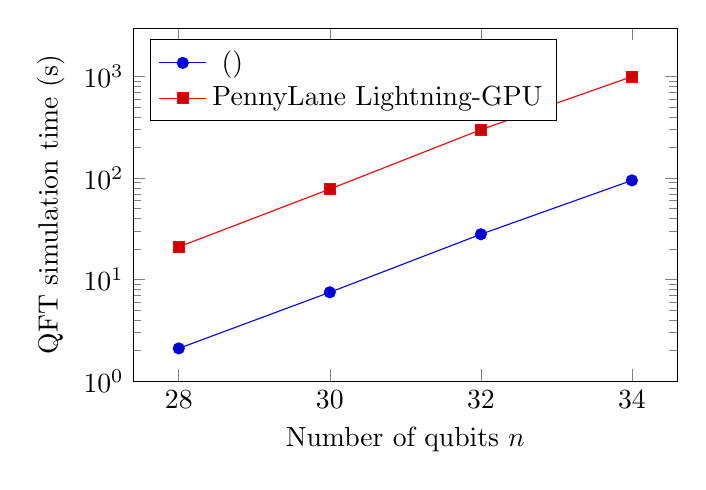
\begin{tikzpicture}
\begin{axis}[
  ymode=log, xlabel={Number of qubits $n$}, ylabel={QFT simulation time (s)},
  xtick={28,30,32,34}, ymin=1, ymax=3000,
  legend pos=north west, legend cell align=left,
  width=0.7\linewidth, height=0.5\linewidth]
  \addplot coordinates {(28,2.1) (30,7.5) (32,28) (34,95)};
  \addlegendentry{\qgear\ (\cudaq)}
  \addplot coordinates {(28,21) (30,78) (32,300) (34,1000)};
  \addlegendentry{PennyLane Lightning-GPU}
\end{axis}
\end{tikzpicture}
\caption{Simulation time of the Quantum Fourier transform versus qubit count for \qgear\ on \cudaq\ and for PennyLane Lightning-GPU on the same A100 hardware (one GPU up to 32 qubits, the four GPUs of one node at 34 qubits). Re-plotted from the approximately $10\times$ advantage reported in \cite{guo2025qgear}; intermediate points are illustrative.}
\label{fig:qgear:qft}
\end{figure}

The VQE benchmark shows the same effect in a variational loop. An 18-qubit VQE instance converged in 126 optimiser iterations to a percent error of \num{2.59e-7} in the ground-state energy. It ran in about \SI{4}{\second} end to end through \qgear\ in adjoint mode, compared with about \SI{10}{\minute} for the same optimisation through the CPU baseline \cite{guo2025qgear}. Each iteration evaluates the expectation values of all Hamiltonian terms on one state. The single-pass \texttt{observe} call of the adjoint mode therefore replaces hundreds of separate circuit executions per iteration. The converged energy agrees with the exact value to the stated precision, which confirms that the transformation preserves the circuit semantics.

\subsection{\qcrank\ Image-Encoding Benchmarks}\label{sec:qgear:results-qcrank}

The final benchmark family targets the data-encoding circuits that recur throughout \cref{ch:qml,ch:synthesis}. \Cref{tab:qgear:qcrank} lists the four images used in \cite{guo2025qgear}, from a $64\times 80$ fingerprint with about 5,000 pixels to a $384\times 256$ zebra with about 98,000 pixels. In \qcrank\ the number of pixels is $2^{n_{a}}n_{d}$, so a given image admits several $(n_{a},n_{d})$ decompositions. The zebra image, for instance, was encoded with 13 address and 12 data qubits, with 14 and 6, and with 15 and 3. Each pixel value is read out from the statistics of its address, so the shot count scales with the number of address states. It ranges from three million shots for the fingerprint to 98 million shots for the 15-address-qubit zebra encoding.

For the smaller images, the GPU pipeline delivered speed-ups approaching two orders of magnitude over the CPU baseline \cite{guo2025qgear}. For the largest shot counts the advantage narrows. The sampling and host-transfer path, not the state-vector update that the GPU accelerates, dominates when $10^{8}$ bit strings are sampled from a 25-qubit state. This observation motivated the multi-shot sampling optimisations discussed in \cref{sec:qgear:discussion} and, more fundamentally, the shot-efficient encodings developed in \cref{ch:qml}.

\begin{table}[htbp]
\caption{\qcrank\ image-encoding benchmarks used in \cite{guo2025qgear}. An image of $2^{n_{a}}\times n_{d}$ pixels is loaded with $n_{a}$ address and $n_{d}$ data qubits; the shot budget grows with the number of address states; the same image can be split between address and data qubits in more than one way. Data from \cite{guo2025qgear}.}
\label{tab:qgear:qcrank}
\centering\small
\begin{threeparttable}
\begin{tabular}{@{}llrccr@{}}
\toprule
Image & Resolution & Pixels & Address qubits $n_{a}$ & Data qubits $n_{d}$ & Shots \\
\midrule
Finger   & $64\times 80$   & 5,120  & 10 & 5  & 3\,M \\
Shoes    & $128\times 128$ & 16,384 & 11 & 8  & 6\,M \\
Building & $192\times 128$ & 24,576 & 12 & 6  & 12\,M \\
Zebra    & $384\times 256$ & 98,304 & 13 & 12 & 24\,M \\
Zebra    & $384\times 256$ & 98,304 & 14 & 6  & 49\,M \\
Zebra    & $384\times 256$ & 98,304 & 15 & 3  & 98\,M \\
\bottomrule
\end{tabular}
\begin{tablenotes}\footnotesize
\item GPU speed-ups over the CPU baseline approach two orders of magnitude for the smaller images \cite{guo2025qgear}.
\end{tablenotes}
\end{threeparttable}
\end{table}

\section{Discussion and Limitations}\label{sec:qgear:discussion}

The results above answer the first half of RQ1 quantitatively. With the GPUs available on a leadership-class system today, exact state-vector simulation reaches 42 qubits. The 30--34-qubit regime that used to require a day of CPU time is now interactive. The design answers the second half of RQ1, usability. No circuit in this chapter was rewritten, and the same HDF5 batch ran on one GPU and on 1,024 GPUs after a change of two lines in a job script. Several limitations bound what this approach can deliver, and they shape the rest of the dissertation.

\emph{The memory wall.} Index-bit partitioning trades memory for GPUs at a fixed exchange rate of one qubit per doubling of the GPU count. With \SI{40}{\giga\byte} per GPU the 1,024 GPUs used here hold 42 qubits. The \SI{80}{\giga\byte} A100 and the newer H100 add one qubit. The entire Perlmutter GPU partition of roughly 7,000 GPUs would add two or three more. Exact simulation of general circuits therefore ends at about 42--45 qubits on any machine that exists or is planned, regardless of software quality.

Beyond that scale, only approximate methods can extend simulation, such as matrix-product states \cite{perezgarcia2006mps} for low-entanglement circuits or the circuit-cutting techniques of \cref{sec:bg:cutting}. They work only when they can exploit structure that random circuits do not have. At this boundary the hardware experiments of \cref{ch:nisq,ch:qml} become the only way to obtain answers. \qgear\ is therefore positioned as a verification and calibration tool for circuits that then run on QPUs, not as a replacement for them.

\emph{Communication for high-order qubits.} Along the memory-limited diagonal of \cref{fig:qgear:scaling} the time per gate rises with $n$. The fraction of gates that touch global qubits grows with $g=n-32$, and each such gate moves half of the distributed state across the network. For random circuits the effect is mild, since global qubits are a small minority. Structured circuits are different: in the QFT or in the address register of \qcrank, a few qubits are addressed by many gates. A fixed qubit ordering can then place a heavily used qubit among the global ones and incur an exchange at nearly every layer. A natural extension is to choose the permutation of logical to index bits so that the most frequently addressed qubits are local, in the spirit of the qubit-reordering strategies in \cite{bayraktar2023cuquantum,doi2023multishotgpu}. The current \qgear\ release leaves this to the \cudaq\ runtime.

\emph{Gate-set coverage.} The eight instructions in \cref{tab:qgear:gates} cover the workloads in this dissertation. They do not cover, for example, multi-controlled gates, arbitrary unitaries given as matrices, mid-circuit measurement with feed-forward, or reset. Some of these are straightforward additions to the dispatch table. Mid-circuit measurement with classical control is not, because it breaks the pure state-vector model on which the multi-GPU partitioning relies. It would require the sampling path of the simulator rather than the state-vector path. The \qawa\ circuits of \cref{ch:nisq}, which use mid-circuit measurement data, were therefore validated with \qgear\ only up to the measurement layer.

\emph{Sampling-dominated workloads.} The \qcrank\ results show the cost of a shallow circuit with a shot count in the tens of millions. The sampling of bit strings from the final state and their transfer to the host then dominate the cost. GPU state-vector acceleration does not address this step. Techniques that sample many shots from a single stored state without a re-simulation of the circuit \cite{doi2023multishotgpu} mitigate this, and \qgear\ uses the multi-shot sampling of \cudaq. The more fundamental remedy is to design encodings that need fewer shots, which is the subject of \cref{ch:qml}.

\emph{Precision.} All results use single-precision complex amplitudes. This halves memory relative to double precision and allows 32 qubits per GPU. For the circuit depths considered here the accumulated rounding error is far below the shot noise of any realistic experiment. The VQE benchmark converged to a relative error of $10^{-7}$. For much deeper circuits, or for small differences of amplitudes, a double-precision target with 31 qubits per GPU is available at twice the memory cost.

\section{Relation to the Other Chapters}\label{sec:qgear:relation}

\qgear\ is the simulation substrate on which the rest of this dissertation stands, and \cref{fig:qgear:relation} shows the concrete connections. The 20-qubit, 10-layer \deal\ circuits of \cref{ch:nisq} were simulated noiselessly through \qgear\ before submission to the IBM Torino and Marrakesh processors. This confirmed that the directly initialised angles reproduced the intended energies. It also gave the noiseless reference distributions used to measure the hardware success probabilities and Kullback--Leibler divergences. The \qawa\ walk circuits of the same chapter were simulated up to 20 qubits with the same pipeline.

% alt: Hub-and-spoke diagram. A Q-GEAR box on the left lists the three-tensor HDF5 encoding, the constant-time kernel builder, the adjoint and parallel modes, the container deployment and exact simulation to 42 qubits. Four arrows lead to boxes on the right, one per later chapter: the NISQ chapter gets noiseless DEAL and QAWA references before QPU runs; the quantum-learning chapter runs ShardQ sub-circuits and QCrank encoders in parallel mode; the AI-synthesis chapter evaluates the RubriQ fidelity reward in CUDA-Q; the QEC chapter starts beyond the memory wall, where verification replaces simulation.
\begin{figure}[htbp]
\centering
\begin{tikzpicture}[
  font=\footnotesize,
  hub/.style={draw,rounded corners=3pt,align=center,fill=cbBlue!15,text width=30mm,minimum height=12mm,inner sep=4pt},
  ch/.style={draw,rounded corners=2pt,align=center,text width=58mm,minimum height=8mm,inner sep=3pt},
  arr/.style={-{Latex[length=2mm]},thick}]
  \node[hub] (hub) at (0,0) {\textbf{\qgear}\\ (this chapter)};
  \node[ch,fill=cbGreen!15]  (c1) at (6.6,2.1)  {\textbf{\Cref{ch:nisq}}: noiseless references};
  \node[ch,fill=cbOrange!15] (c2) at (6.6,0.7)  {\textbf{\Cref{ch:qml}}: sub-circuit simulation};
  \node[ch,fill=cbPurple!15] (c3) at (6.6,-0.7) {\textbf{\Cref{ch:synthesis}}: fidelity reward};
  \node[ch,fill=cbRed!15]    (c4) at (6.6,-2.1) {\textbf{\Cref{ch:qec}}: verification beyond the memory wall};
  \draw[arr] (hub.east) -- (c1.west);
  \draw[arr] (hub.east) -- (c2.west);
  \draw[arr] (hub.east) -- (c3.west);
  \draw[arr] (hub.east) -- (c4.west);
\end{tikzpicture}
\caption{How \qgear\ feeds the later chapters. Schematic.}
\label{fig:qgear:relation}
\end{figure}

In \cref{ch:qml} the \shardq\ circuit-cutting framework knits sub-circuit results on A100 GPUs. The cost of its quasi-probability reconstruction grows as $3^{2k}$ in the number of cuts $k$. The parallel mode of \cref{sec:qgear:modes} ran the sub-circuit simulations and made this reconstruction tractable. The \qcrank\ encoders benchmarked in \cref{tab:qgear:qcrank} are the same encoders that \shardq\ cuts and that \vqt\ uses for its vectorised attention. In \cref{ch:synthesis} the \rubriq\ reinforcement-learning loop simulates every generated circuit in \cudaq\ to evaluate the fidelity component of its rubric reward. The constant-time kernel construction and the container deployment allow thousands of candidate circuits per training step on the Perlmutter nodes that host the language model.

Finally, the memory wall of \cref{sec:qgear:discussion} is why the later chapters turn from simulating quantum computation to trusting it. Once circuits exceed what any classical machine can check, the questions of \cref{ch:qec} about auditable error correction on shared hardware become unavoidable.

\section{Summary}\label{sec:qgear:summary}

This chapter presented \qgear, a framework that makes GPU-accelerated state-vector simulation available to \qiskit\ users without a rewrite of their circuits. The framework has four parts:
\begin{itemize}
  \item a three-tensor HDF5 encoding that decouples circuit generation from execution;
  \item a constant-time kernel transformation over a compact but universal gate set;
  \item adjoint and parallel modes for the two shapes of HPC quantum workloads;
  \item a containerised, Slurm-integrated deployment that partitions one state vector across GPUs by index-bit decomposition, so that the same job script runs on one GPU or on 1,024.
\end{itemize}
Experiments reported in \cite{guo2025qgear} showed:
\begin{itemize}
  \item roughly two orders of magnitude speed-up over a 128-core CPU node, with a 34-qubit random unitary reduced from about a day to about a minute on one GPU node;
  \item roughly one order of magnitude over existing GPU simulators, with 20--100$\times$ gains on the QFT;
  \item an 18-qubit VQE reduced from ten minutes to four seconds;
  \item exact simulation of 42-qubit circuits on 1,024 A100 GPUs at near-full utilisation.
\end{itemize}
The chapter also identified the limits of the approach: a memory wall at about 42--45 qubits, communication costs for heavily used global qubits, a restricted gate set, and sampling-dominated encoding workloads. These limits motivate the hardware-aware algorithms of \cref{ch:nisq}, the shot-efficient encodings of \cref{ch:qml}, and the verification questions of \cref{ch:qec}. The pipeline itself remains the tool with which every circuit in those chapters was first validated.
